\documentclass[table, usenames, svgnames, dvipsnames]{beamer}
\usepackage{listings}
\usepackage{beamerthemeshadow}
\usepackage[latin1]{inputenc}
\usepackage[absolute,overlay]{textpos}
\usepackage{array}

% Coisas adicionadas pelo Alberto.
\usepackage{proof}
\usepackage{easylist}
% \usepackage[portuguese]{babel}
\usepackage{amsmath}
\usepackage[round]{natbib}

\usepackage{verbatim}

\usetheme{Rochester}
%\usetheme{Luebeck}
\usecolortheme{rose}

\setbeamerfont{frametitle}{size=\normalsize}
\setbeamerfont{title}{size=\normalsize}
\beamertemplatenavigationsymbolsempty

\setbeamertemplate{navigation symbols}{}
\setbeamertemplate{footline}{}

\DeclareGraphicsExtensions{.pdf,.jpg,.png} % compilamos apenas com pdflatex
\graphicspath{{.}{./figuras/}} % caminho onde as figuras estarao disponiveis

\setlength{\TPHorizModule}{1mm}

\setlength{\TPVertModule}{1mm}
\newcommand{\MyLogo}{%
\begin{textblock}{}(118.5, 2.5)
   \includegraphics[width=0.7cm]{figuras/ime-mod2.png}
\end{textblock}
}

\title{\footnotesize Automa��o de Testes em Aplica��es de BPMS: um Relato de Experi�ncia}

% \usepackage{framed} % utilizado para codigo fonte
\definecolor{shadecolor}{named}{LightGray}

\usepackage[portuguese]{babel}

% ---------------------------------------------------------------------------- %
% T�tulo
% ---------------------------------------------------------------------------- %

\subtitle{}
\date{}

% ---------------------------------------------------------------------------- %
\begin{document}
% ---------------------------------------------------------------------------- %

% ---------------------------------------------------------------------------- %
% Primeira p�gina: slide 0
% --------------------------------------------------------------------------- - %
\begin{frame}
   \centering
   \textsc{Universidade Federal de Santa Maria}\\
   \textsc{Programa de P�s-Gradua��o em Inform�tica - PPGI}\\
   \vspace{15pt}
   \titlepage
   \vspace{-60pt}
   \begin{center}
      \textsc{}\\
      \textsc{}\\
      \hfill\\
      \textsc{} J�ssica Lasch de Moura e Andrea Schwertner Char�o
   \end{center}
\end{frame}

\begin{frame}
\frametitle{Introdu��o} 
\begin{itemize}
\item BPM e BPMS;
\item Verifica��o e testes = desafio;
\begin{itemize}
\item Falta de automa��o nos testes pode levar a problemas.
\end{itemize}
\end{itemize}
  \begin{figure}[h]
    \centering
    
\includegraphics[height=0.3\paperheight]{figuras/bpm-engine.jpg}
    %\includegraphics[height=6cm]{figCoordEsf02}
%    \caption{}
  \end{figure}
\end{frame}

\begin{frame}
\frametitle{BPM e Testes} 
\begin{itemize}
\item Ciclo de vida BPM
\end{itemize}
  \begin{figure}[h]
    \centering
    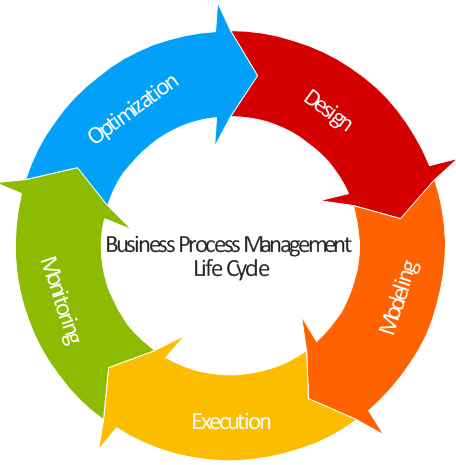
\includegraphics[height=0.6\paperheight]{figuras/bpm-lyfe-cycle.png}
    %\includegraphics[height=6cm]{figCoordEsf02}
    \caption{Ciclo de vida BPM. Fonte: https://conceptdraw.com}
  \end{figure}
\end{frame}

\begin{frame}
\frametitle{BPM e Testes} 
\begin{itemize}
\item estudar o que colocar nesse slide!
\end{itemize}
\end{frame}

\begin{frame}
\frametitle{Aplica��o alvo dos testes} 
  \begin{figure}[h]
    \centering
    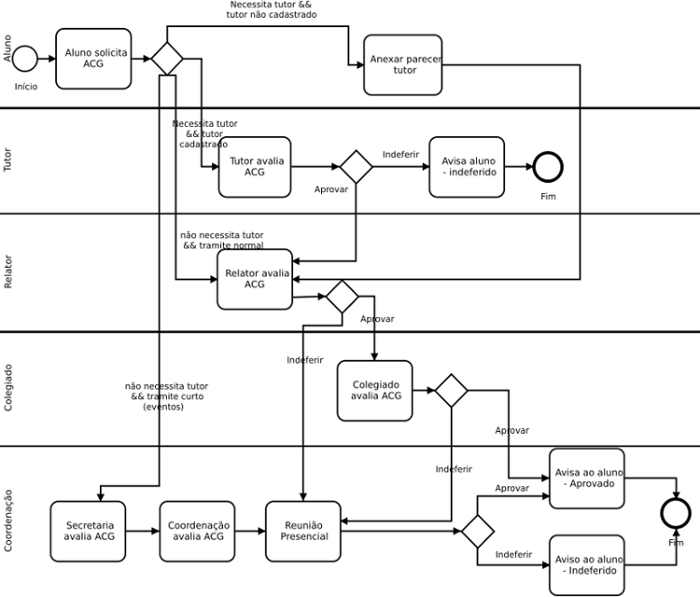
\includegraphics[height=0.65\paperheight]{figuras/processo.png}
    %\includegraphics[height=6cm]{figCoordEsf02}
    \caption{Processo alvo dos testes: Solicita��o de Atividade Complementar de Gradua��o}
  \end{figure}
\end{frame}

\begin{frame}
\frametitle{Aplica��o alvo dos testes} 
\begin{itemize}
\item A aplica��o foi submetida a testes funcionais realizados manualmente;
\item BPMS utilizado n�o possu�a suporte a nenhum tipo de teste automatizado;
\item Buscou-se outros BPMS com licen�as open source ou freeware, que pudessem implementar o processo em quest�o e que oferecessem suporte a testes.
\end{itemize}
  \begin{figure}[h]
    \centering
    
\includegraphics[width=0.7\paperwidth]{figuras/bpms.png}
    %\includegraphics[height=6cm]{figCoordEsf02}
    \caption{BPMS analisados}
  \end{figure}
\end{frame}


%Se��o 15.4 e 16.4
\begin{frame}
\frametitile{Bibliografia}
\bibliographystyle{sbc}
\bibliography{sbc-template}
\end{frame}
%\bibliography{referencias}
%\bibliographystyle{plainnat}

\end{document}
